\section{Intra-domain Routing Protocol: IS-IS}
\label{sec:isis}

\subsection{Design}

Due to the limitation of the static routing, routers cannot find alternative paths if a set path is broken and thus a new path need to be set manually. 
In contrast, dynamic routing always finds the least cost path even when the previous least cost path is broken.
Popular dynamic routing protocols include distance vector based protocols like RIP and link state based protocols like IS-IS and OSPF. 

In this lab, the IS-IS is used as the Interior Gateway Protocol (IGP), which provides faster convergence and larger scalability compared to distance vector based protocols. 
IS-IS is short for Intermediate System to Intermediate System Routing Protocol.
By using this protocol, each router maintains a database which has a map of the whole topology and all routers have the same information. The best path to every destination is computed by all routers. 
Figure \ref{fig:isis} shows the design of IS-IS protocol in BT Network. As the figure shows, the network only has level-1 routers for internal routing.

\begin{figure}[ht!]
    \centering
    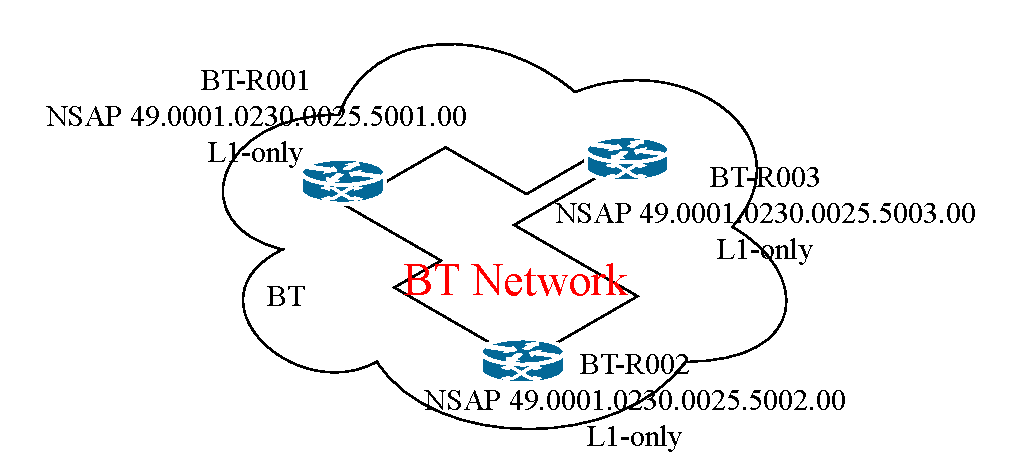
\includegraphics[width=\linewidth]{isis}
    \caption{Design of IS-IS Protocol in BT Network.}
    \label{fig:isis}
\end{figure}

\subsection{Loopback Addresses and NSAP for Routers}

To set up IS-IS, an unique loopback address is needed for each router. 
An IPv4 address block of \texttt{23.0.255.0/24} and IPv6 address block of \texttt{2001:2300:ffff::/48} is allocated for loopback addresses. 

Following the CLNS addressing convention, each router is then assigned with a NSAP. A NSAP has $3$ main components. 

According to the convention, the leading Area ID is composed of AFI ($49$) and Area Address ($0001$). 
The System ID followed is set to the IPv4 loopback address of the router. If the loopback address is $ABC.DEF.GHI.JKL$, then System ID should be $ABCD.EFGH.IJKL$.
The last main component is N-Selector (NSEL) and set to $00$.

The assignment of addresses and NSAP to routers are detailed in Table \ref{tab:isis}.

\begin{longtable}[]{@{}llll@{}}
\toprule
Router & IPv4 Loopback Address & IPv6 Loopback Address & NSAP\tabularnewline
\midrule
\endhead
BT-R001 & 23.0.255.1 & 2001:2300:ffff:1:: & 49.0001.0230.0025.5001.00\tabularnewline
BT-R002 & 23.0.255.2 & 2001:2300:ffff:2:: & 49.0001.0230.0025.5002.00\tabularnewline
BT-R003 & 23.0.255.3 & 2001:2300:ffff:3:: & 49.0001.0230.0025.5003.00\tabularnewline
\bottomrule
\caption{IP Loopback Addresses and NSAP for Routers in BT Network.}
\label{tab:isis}
\end{longtable}



\subsection{Implementation}

IS-IS is set up on Router 1 (BT-R001) using the following commands.

\begin{lstlisting}
interface Loopback0
ip address 23.0.255.1 255.255.255.255
ipv6 address 2001:2300:FFFF:1::/128

router isis
net 49.0001.0230.0025.5001.00
is-type level-1
\end{lstlisting}

Then, IS-IS is turned on on all interfaces to internal routers.

\begin{lstlisting}
interface FastEthernet0/0
ip router isis
ipv6 router isis

interface FastEthernet0/1
ip router isis
ipv6 router isis

interface FastEthernet0/1/0
ip router isis
ipv6 router isis
\end{lstlisting}

\clearpage

However, IS-IS routes should not be broadcasted nor received through the loopback interface (\texttt{Loopback0}) while the route to corresponding subnet should be broadcasted to other internal routers. Therefore, the loopback interface should be a passive interface in IS-IS protocol.

\begin{lstlisting}
router isis
passive-interface Loopback0
\end{lstlisting}

For Router 2 (BT-R002) and Router 3 (BT-R002), IS-IS is set up similarly using the above commands. The main difference is that interfaces to external routers (VLAN 3 for Router 2 and VLAN 4 \& 5 for Router 3) should be passive interfaces as well. Below is the configuration for Router 2.

\begin{lstlisting}
interface Loopback0
ip address 23.0.255.2 255.255.255.255
ipv6 address 2001:2300:FFFF:2::/128

router isis
net 49.0001.0230.0025.5002.00
is-type level-1
passive-interface Vlan3
passive-interface Loopback0

interface FastEthernet0/0
ip router isis
ipv6 router isis

interface FastEthernet0/1
ip router isis
ipv6 router isis

interface Vlan1
ip router isis
ipv6 router isis
\end{lstlisting}

Below is the configuration for Router 3.

\begin{lstlisting}
interface Loopback0
ip address 23.0.255.3 255.255.255.255
ipv6 address 2001:2300:FFFF:3::/128

router isis
net 49.0001.0230.0025.5003.00
is-type level-1
passive-interface Vlan4
passive-interface Vlan5
passive-interface Loopback0

interface FastEthernet0/0
ip router isis
ipv6 router isis

interface FastEthernet0/1
ip router isis
ipv6 router isis

interface Vlan2
ip router isis
ipv6 router isis
\end{lstlisting}


\subsection{Evaluation}

Once the IS-IS is set up, use \texttt{traceroute} command to check the IPv4 path from Laptop 1 (BT001, IPv4 Address: \texttt{23.0.0.2}) to Laptop 2 (BT002, IPv4 Address: \texttt{23.0.0.18}) in the network.

\begin{lstlisting}[language=sh]
traceroute 23.0.0.34
\end{lstlisting}

Figure \ref{fig:isis-traceroute} shows the route taken is 
\texttt{Laptop 1 (BT001, IPv4 Address: 23.0.0.2)
-> Router 1 (BT-R001, IPv4 Address: 23.0.0.1) 
-> Router 2 (BT-R002, IPv4 Address: 23.0.0.50)
-> Laptop 2 (BT002, IPv4 Address: 23.0.0.18)}, which is a correct route.
Routes from Laptop 1 to Laptop 3 as well as from Laptop 2 to Laptop 3 are tested and shown in the figure as well.

\begin{figure}[ht!]
    \centering
    \begin{subfigure}[b]{\textwidth}
        \centering
        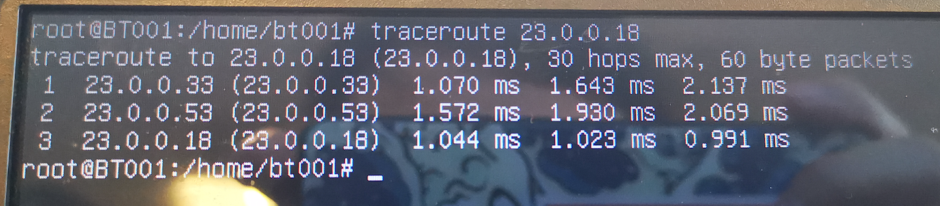
\includegraphics[width=\linewidth]{isis-traceroute-1-2}
        \caption{\texttt{traceroute} from Laptop 1 (BT001) to Laptop 2 (BT002)}
    \end{subfigure}
    ~
    \begin{subfigure}[b]{\textwidth}
        \centering
        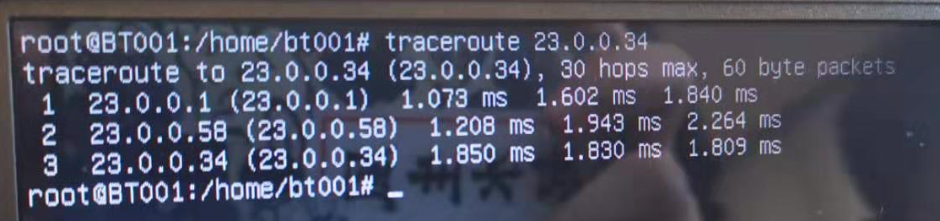
\includegraphics[width=\linewidth]{isis-traceroute-1-3}
        \caption{\texttt{traceroute} from Laptop 1 (BT001) to Laptop 3 (BT003)}
    \end{subfigure}
    ~
    \begin{subfigure}[b]{\textwidth}
        \centering
        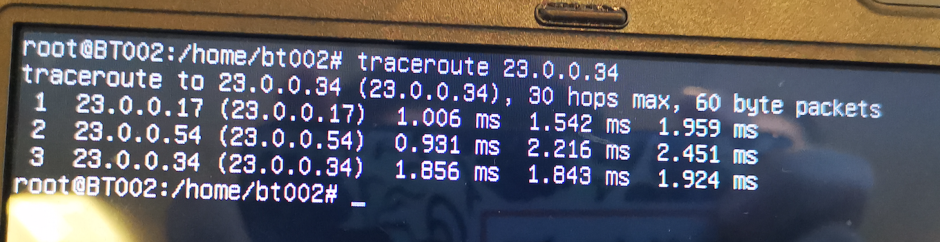
\includegraphics[width=\linewidth]{isis-traceroute-2-3}
        \caption{\texttt{traceroute} from Laptop 2 (BT002) to Laptop 3 (BT003)}
    \end{subfigure}
    \caption{Tracing IPv4 Routes between Laptops using \texttt{traceroute}.}
    \label{fig:isis-traceroute}
\end{figure}

Similiar results can be observed for IPv6 routes in Figure \ref{fig:isis-traceroute-ipv6}. The IPv6 Route taken from Laptop 1 to Laptop 2 is 
\texttt{Laptop 1 (BT001, IPv6 Address: 2001:2300::2)
-> Router 1 (BT-R001, IPv6 Address: 2001:2300::1) 
-> Router 2 (BT-R002, IPv6 Address: 2001:2300:3:2::2)
-> Laptop 2 (BT002, IPv6 Address: 2001:2300:0:1::2)}, , which is also a correct route.
Routes from Laptop 1 to Laptop 3 as well as from Laptop 2 to Laptop 3 are tested and shown in the figure as well.


\begin{figure}[ht!]
    \centering
    \begin{subfigure}[b]{\textwidth}
        \centering
        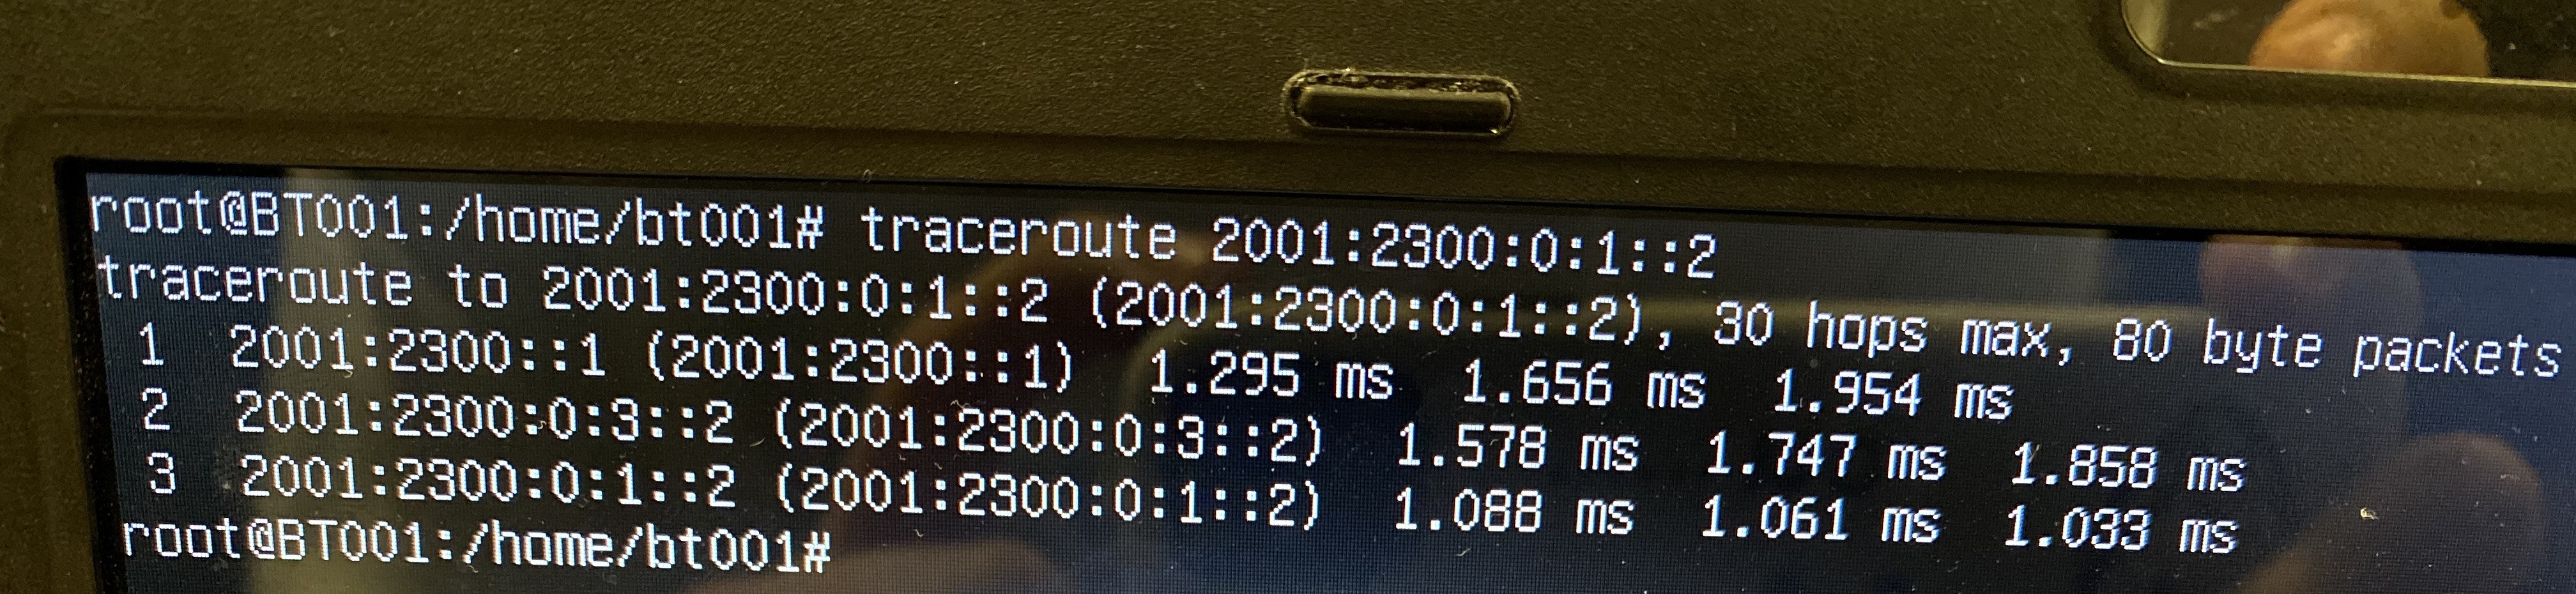
\includegraphics[width=\linewidth]{isis-traceroute-ipv6-1-2}
        \caption{\texttt{traceroute} from Laptop 1 (BT001) to Laptop 2 (BT002)}
    \end{subfigure}
    ~
    \begin{subfigure}[b]{\textwidth}
        \centering
        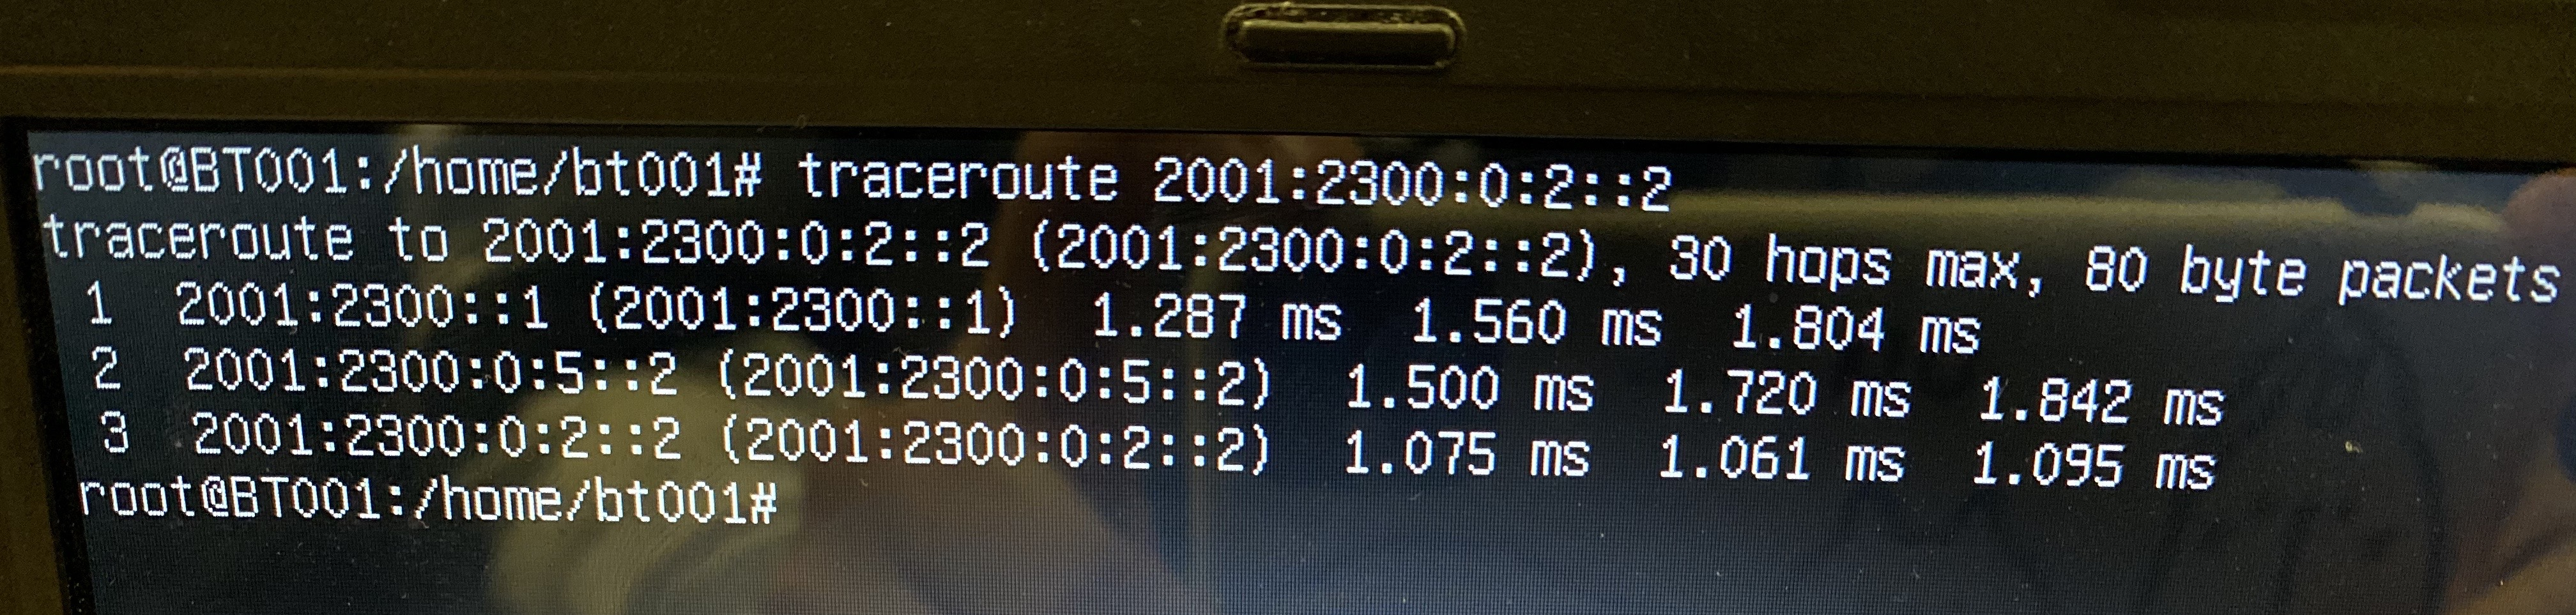
\includegraphics[width=\linewidth]{isis-traceroute-ipv6-1-3}
        \caption{\texttt{traceroute} from Laptop 1 (BT001) to Laptop 3 (BT003)}
    \end{subfigure}
    ~
    \begin{subfigure}[b]{\textwidth}
        \centering
        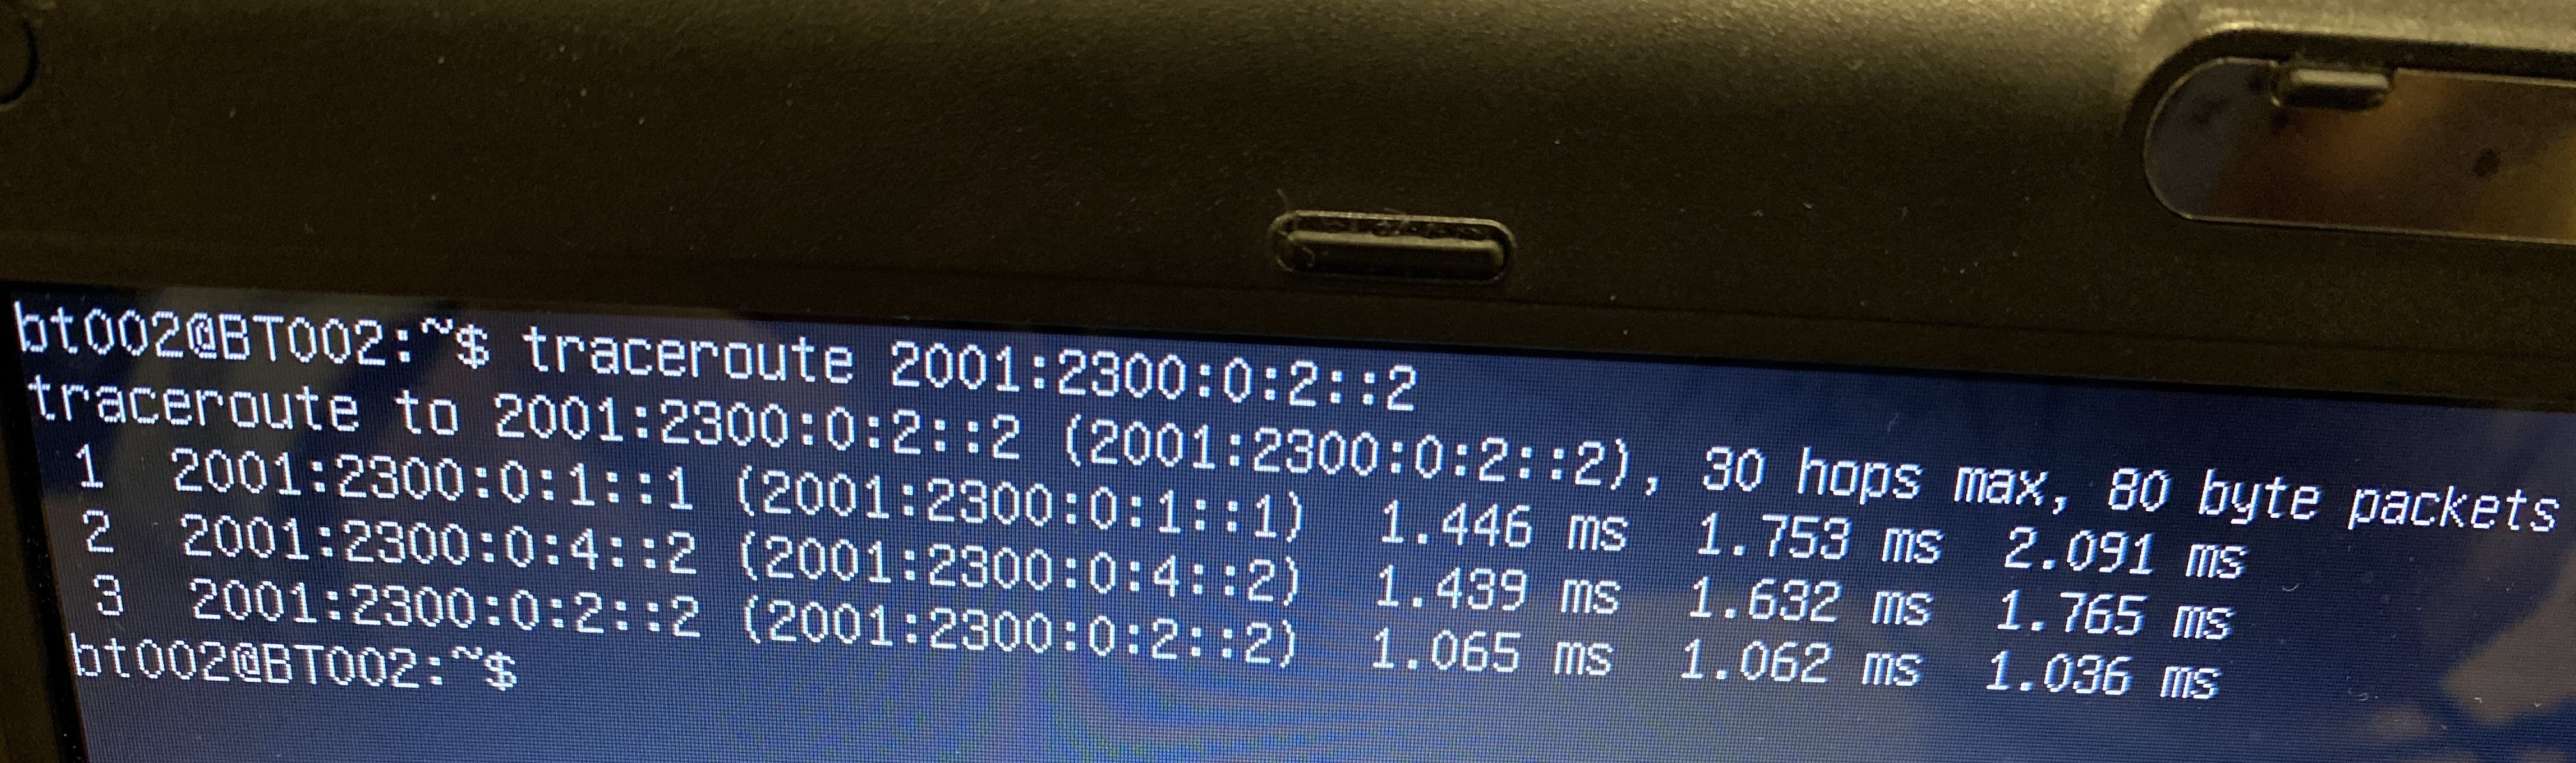
\includegraphics[width=\linewidth]{isis-traceroute-ipv6-2-3}
        \caption{\texttt{traceroute} from Laptop 2 (BT002) to Laptop 3 (BT003)}
    \end{subfigure}
    \caption{Tracing IPv6 Routes between Laptops using \texttt{traceroute}.}
    \label{fig:isis-traceroute-ipv6}
\end{figure}

\clearpage

To further evaluate the correctness of our implementation, we check the path from Laptop 1 to Laptop 2 under the condition that the physical connection between Router 1 and Router 2 is broken. The IS-IS protocol on Router 1 should be able to find route to Router 2 through Router 3.

Figure \ref{fig:isis-traceroute-broken} shows the IPv4 route taken is 
\texttt{Laptop 1 (BT001, IPv6 Address: 23.0.0.2)
-> Router 1 (BT-R001, IPv4 Address: 23.0.0.1) 
-> Router 3 (BT-R003, IPv4 Address: 23.0.0.58) 
-> Router 2 (BT-R002, IPv4 Address: 23.0.0.53)
-> Laptop 2 (BT002, IPv4 Address: 23.0.0.18)}, which is a correct route.


\begin{figure}[ht!]
    \centering
    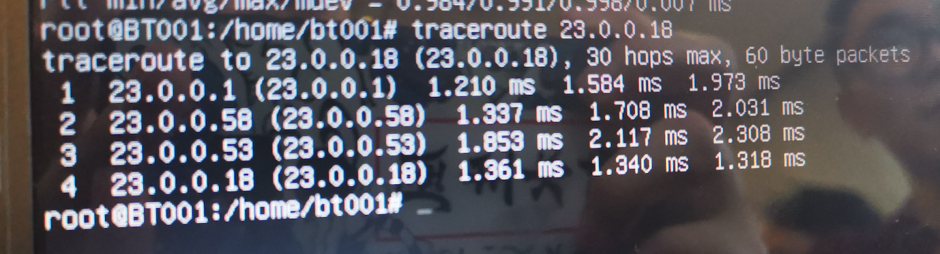
\includegraphics[width=0.8\linewidth]{isis-traceroute-broken-1-2}
    \caption{Tracing IPv4 Routes from Laptop 2 (BT002) to Laptop 3 (BT003) when Physical Connection between Router 1 (BT-R001) and Router 2 (BT-R002) is broken.}
    \label{fig:isis-traceroute-broken}
\end{figure}

Figure \ref{fig:isis-traceroute-broken-ipv6} shows the IPv6 route taken is 
\texttt{Laptop 1 (BT001, IPv6 Address: 2001:2300::2)
-> Router 1 (BT-R001, IPv6 Address: 2001:2300::1) 
-> Router 3 (BT-R003, IPv6 Address: 2001:2300:0:5::2) 
-> Router 2 (BT-R002, IPv6 Address: 2001:2300:0:4::1)
-> Laptop 2 (BT002, IPv6 Address: 2001:2300:0:1::2)}, which is also a correct route.

\begin{figure}[ht!]
    \centering
    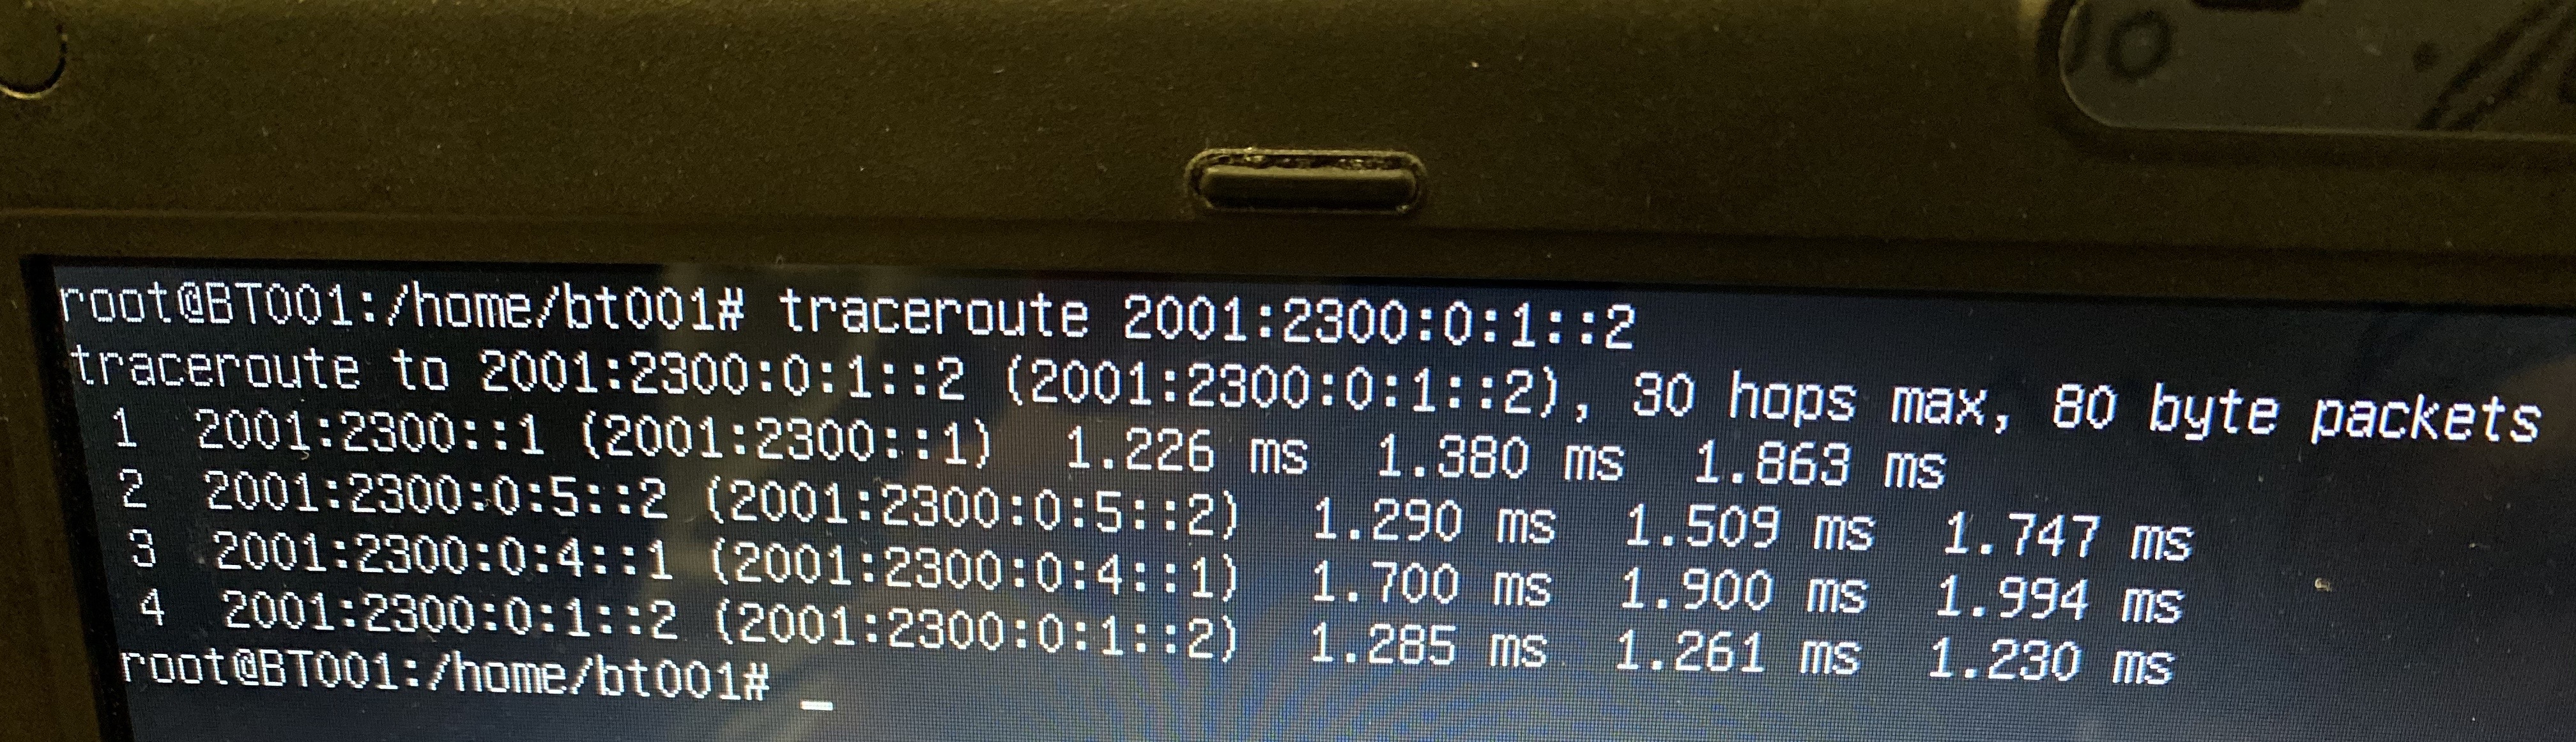
\includegraphics[width=0.8\linewidth]{isis-traceroute-broken-ipv6-1-2}
    \caption{Tracing IPv6 Routes from Laptop 2 (BT002) to Laptop 3 (BT003) when Physical Connection between Router 1 (BT-R001) and Router 2 (BT-R002) is broken.}
    \label{fig:isis-traceroute-broken-ipv6}
\end{figure}

\clearpage

On the router's side, \texttt{show ip route} and \texttt{show ipv6 route} is used to inspect the routes discovered by IS-IS protocol. In Figure \ref{fig:isis-ip-route} and \ref{fig:isis-ipv6-route}, such routes to other subnets inside BT Network on each router are shown.

\begin{figure*}[ht!]
    \centering
    \begin{subfigure}[b]{0.67\textwidth}
        \centering
        \includegraphics[width=\linewidth]{isis-ip-route-1}
        \caption{Router 1 (BT-R001)}
    \end{subfigure}
    \hfill
    \begin{minipage}[b]{0.3\textwidth}
	    \begin{subfigure}[b]{\linewidth}
	        \centering
	        \includegraphics[width=\linewidth]{isis-ip-route-2}
	        \caption{Router 2 (BT-R002)}
	    \end{subfigure}
	    \\
	    \begin{subfigure}[b]{\linewidth}
	        \centering
	        \includegraphics[width=\linewidth]{isis-ip-route-3}
	        \caption{Router 3 (BT-R003)}
	    \end{subfigure}
	\end{minipage}
    \caption{IPv4 Routes to Other Subnets on All $3$ Routers Respectively using \texttt{show ip route}.}
    \label{fig:isis-ip-route}
\end{figure*}


\begin{figure*}[ht!]
    \centering
    \begin{subfigure}[b]{0.67\textwidth}
        \centering
        \includegraphics[width=\linewidth]{isis-ipv6-route-1}
        \caption{Router 1 (BT-R001)}
    \end{subfigure}
    \hfill
    \begin{minipage}[b]{0.3\textwidth}
	    \begin{subfigure}[b]{\linewidth}
	        \centering
	        \includegraphics[width=\linewidth]{isis-ipv6-route-2}
	        \caption{Router 2 (BT-R002)}
	    \end{subfigure}
	    \\
	    \begin{subfigure}[b]{\linewidth}
	        \centering
	        \includegraphics[width=\linewidth]{isis-ipv6-route-3}
	        \caption{Router 3 (BT-R003)}
	    \end{subfigure}
	\end{minipage}
    \caption{IPv6 Routes to Other Subnets on All $3$ Routers Respectively using \texttt{show ipv6 route}.}
    \label{fig:isis-ipv6-route}
\end{figure*}

\clearpage

Noticably, when the physical connection between Router 1 and Router 2 is broken, the route from Router 1 to Router 2 goes through Router 3 instead, as evident in Figure \ref{fig:isis-ip-route-broken}.

\begin{figure}[ht!]
    \centering    
    \begin{subfigure}[b]{\textwidth}
        \centering
        \includegraphics[width=\linewidth]{isis-ip-route-broken-1}
        \caption{IPv4 Routes to Other Subnets on Router 1 using \texttt{show ip route}.}
    \end{subfigure}
    ~
    \begin{subfigure}[b]{\textwidth}
        \centering
        \includegraphics[width=\linewidth]{isis-ipv6-route-broken-1}
        \caption{IPv6 Routes to Other Subnets on Router 1 using \texttt{show ip route}.}
    \end{subfigure}
    \caption{IP Routes to Other Subnets on Router 1 when Physical Connection between Router 1 (BT-R001) and Router 2 (BT-R002) is broken.}
    \label{fig:isis-ip-route-broken}
\end{figure}

\subsection{Commentary}

\subsubsection{Problem: IS-IS Not Set Up for Laptop-Router Interface}
When initially setting up IS-IS on the interfaces, only the interfaces between routers have been turned on. This leads to laptop's failure to reach a router not directly connected.
To solve this problem, IS-IS is set up on the interface between a laptop and a router.

\subsubsection{Alternative Solution to Passive Interfaces}
While turning interfaces connected to outside network into passive interfaces does enable other routers in the network to connect to outside networks through those interfaces, it demands extra computing resource for computing routes to external subnets. 

\textbf{Alternatively, one can disable IS-IS on such interfaces and replace the external next-hop for each out-going route in BGP with the internal router to which the next-hop is directly connected to. That prevents Router-Neighbour subnet from participating in IS-IS routing and eliminates the extra computing consumption while preserving the connectivity between internal routers and outside networks.}


\clearpage



